\chapter{Supporting material for ``Evaluating trait databases for taxon set enrichment analysis"}
\section{Supplemental Figures}

\begin{figure}
    \centering
    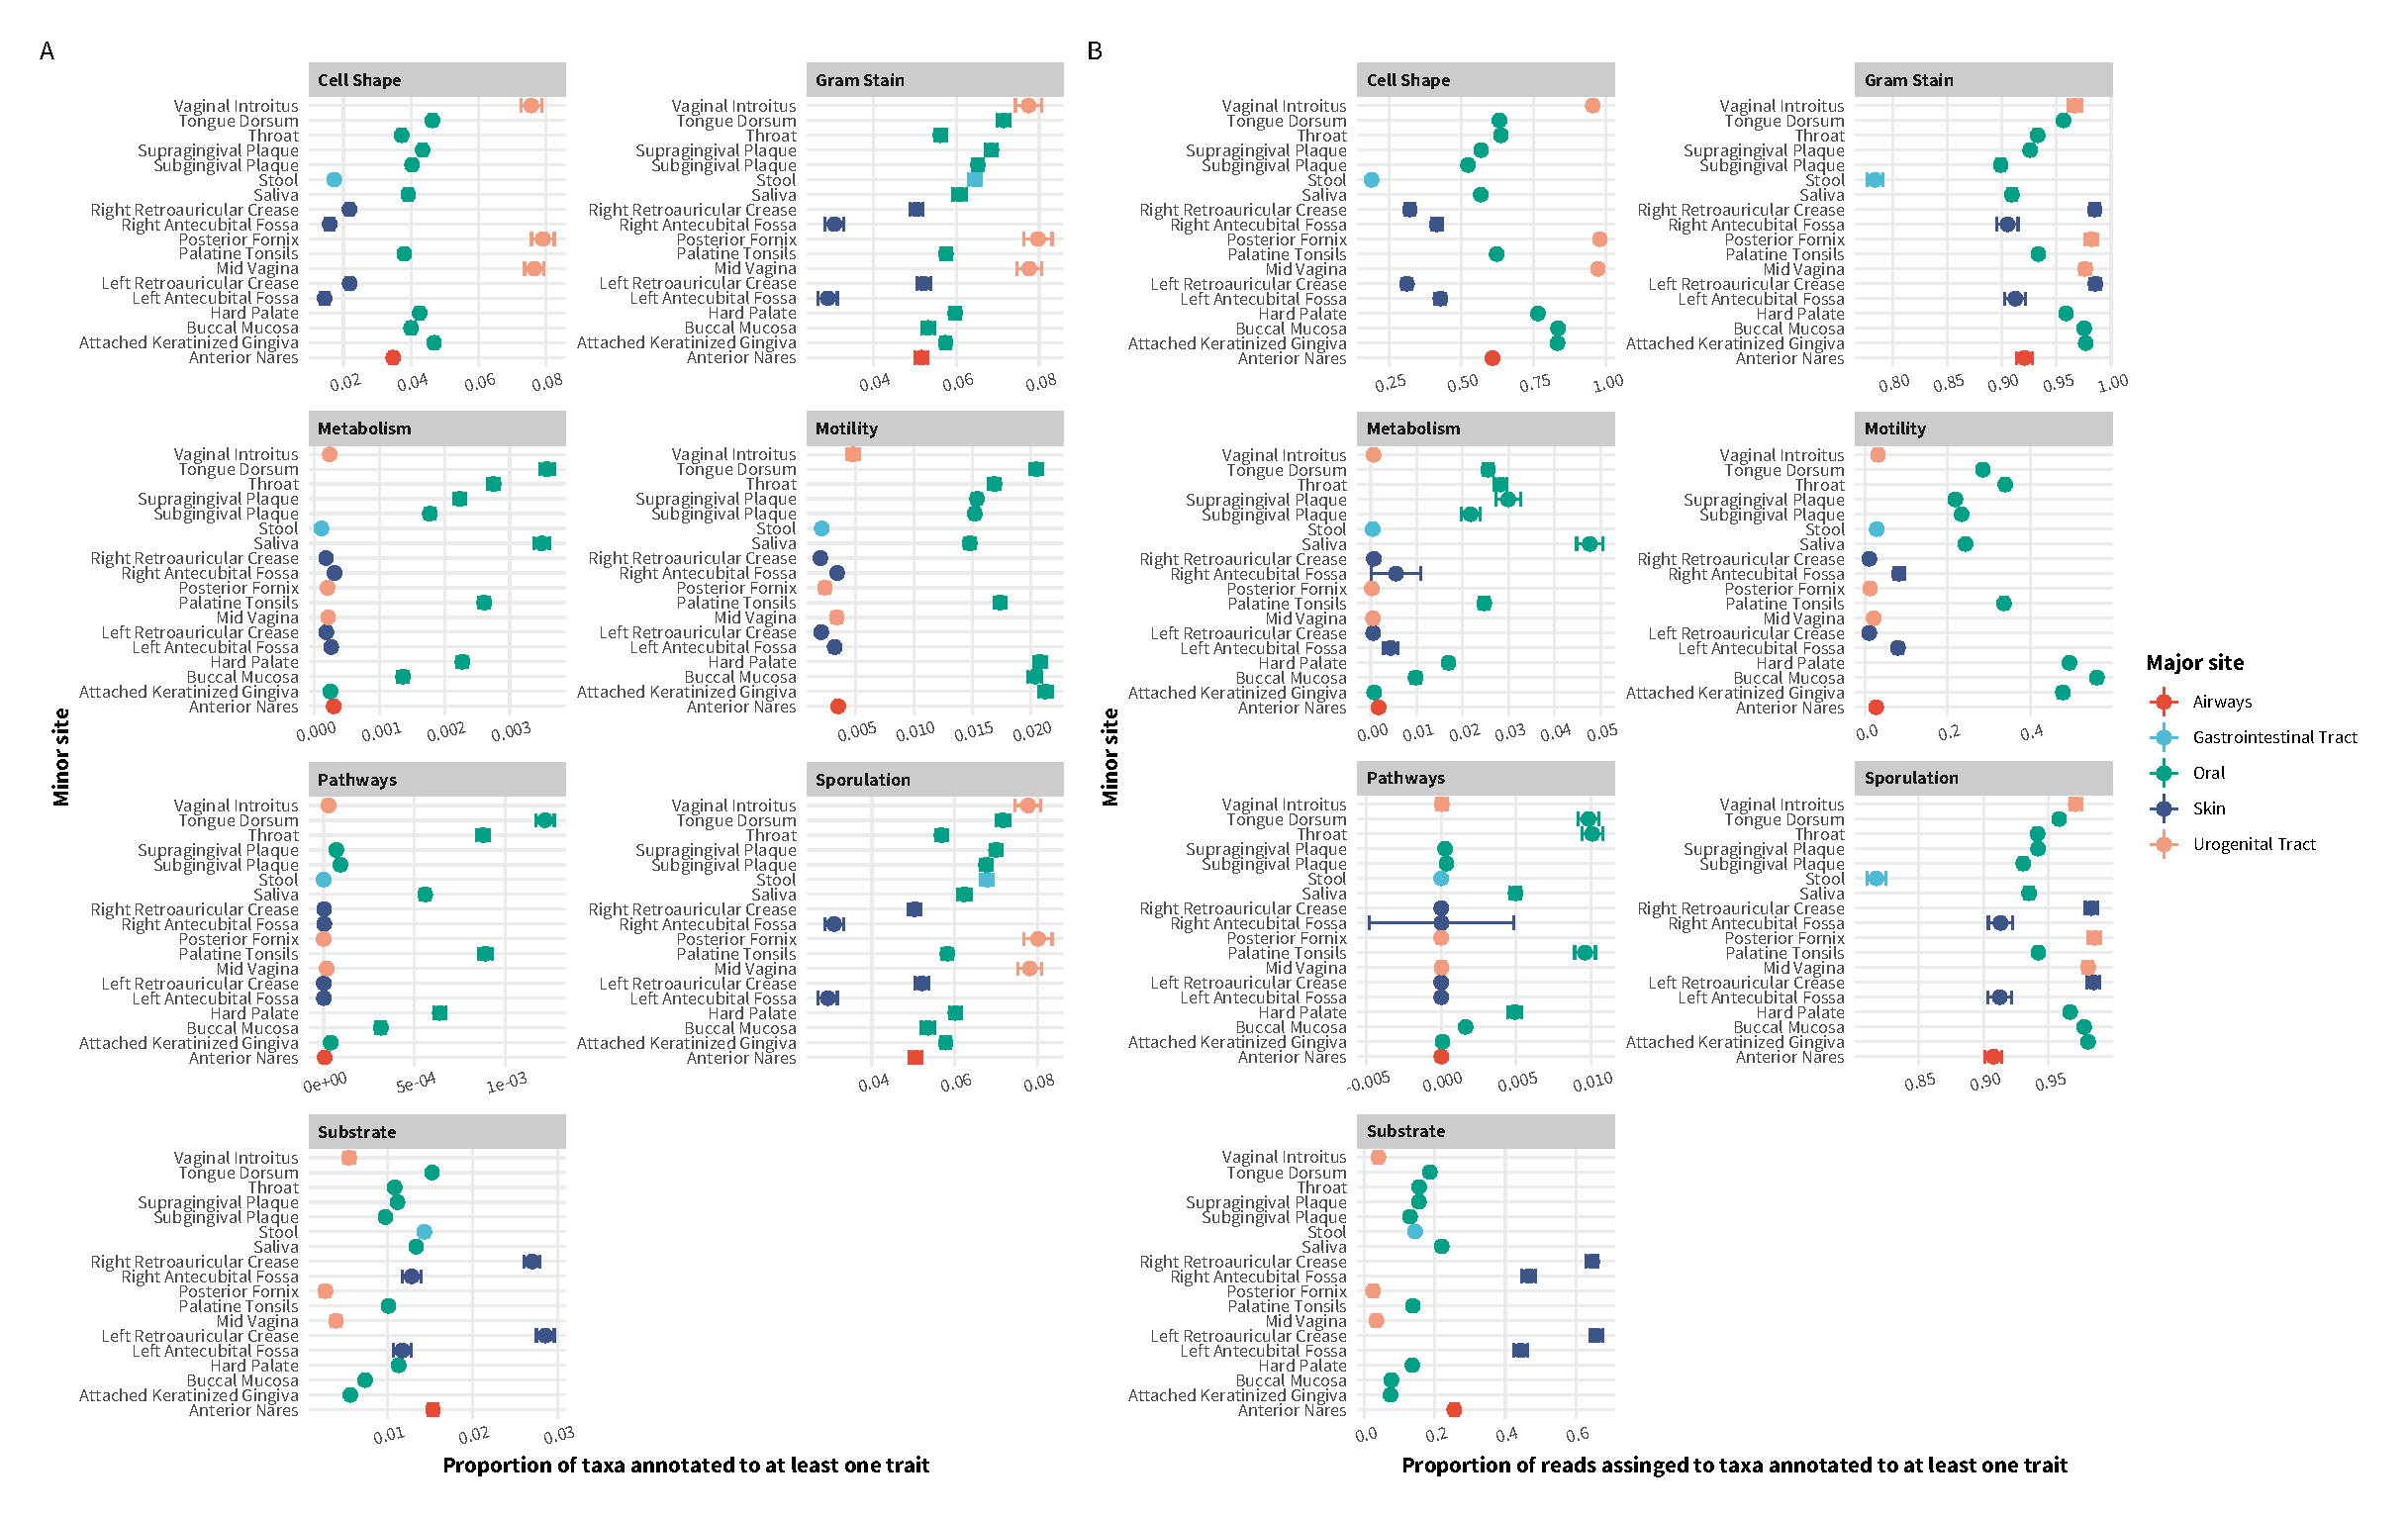
\includegraphics[width=\linewidth]{figures/appD_fs1.eps}
    \caption[Trait coverage statistics for samples profiled with 16S rRNA gene metabarcoding]{Trait coverage statistics for samples profiled with 16S rRNA gene metabarcoding. Panel \textbf{(A)} illustrates the proportion of present taxa per sample annotated to at least one trait. Panel \textbf{(B)} illustrates the proportion of reads assigned to taxa annotated to at least one trait which accounts for taxa relative abundances. Each plot facet represents different trait categories that were evaluated. Error bar represents the standard error of the evaluation statistic of interest across the the total number of samples evaluated per body site.}
    \label{fig:d1}
\end{figure}

\begin{figure}
    \centering
    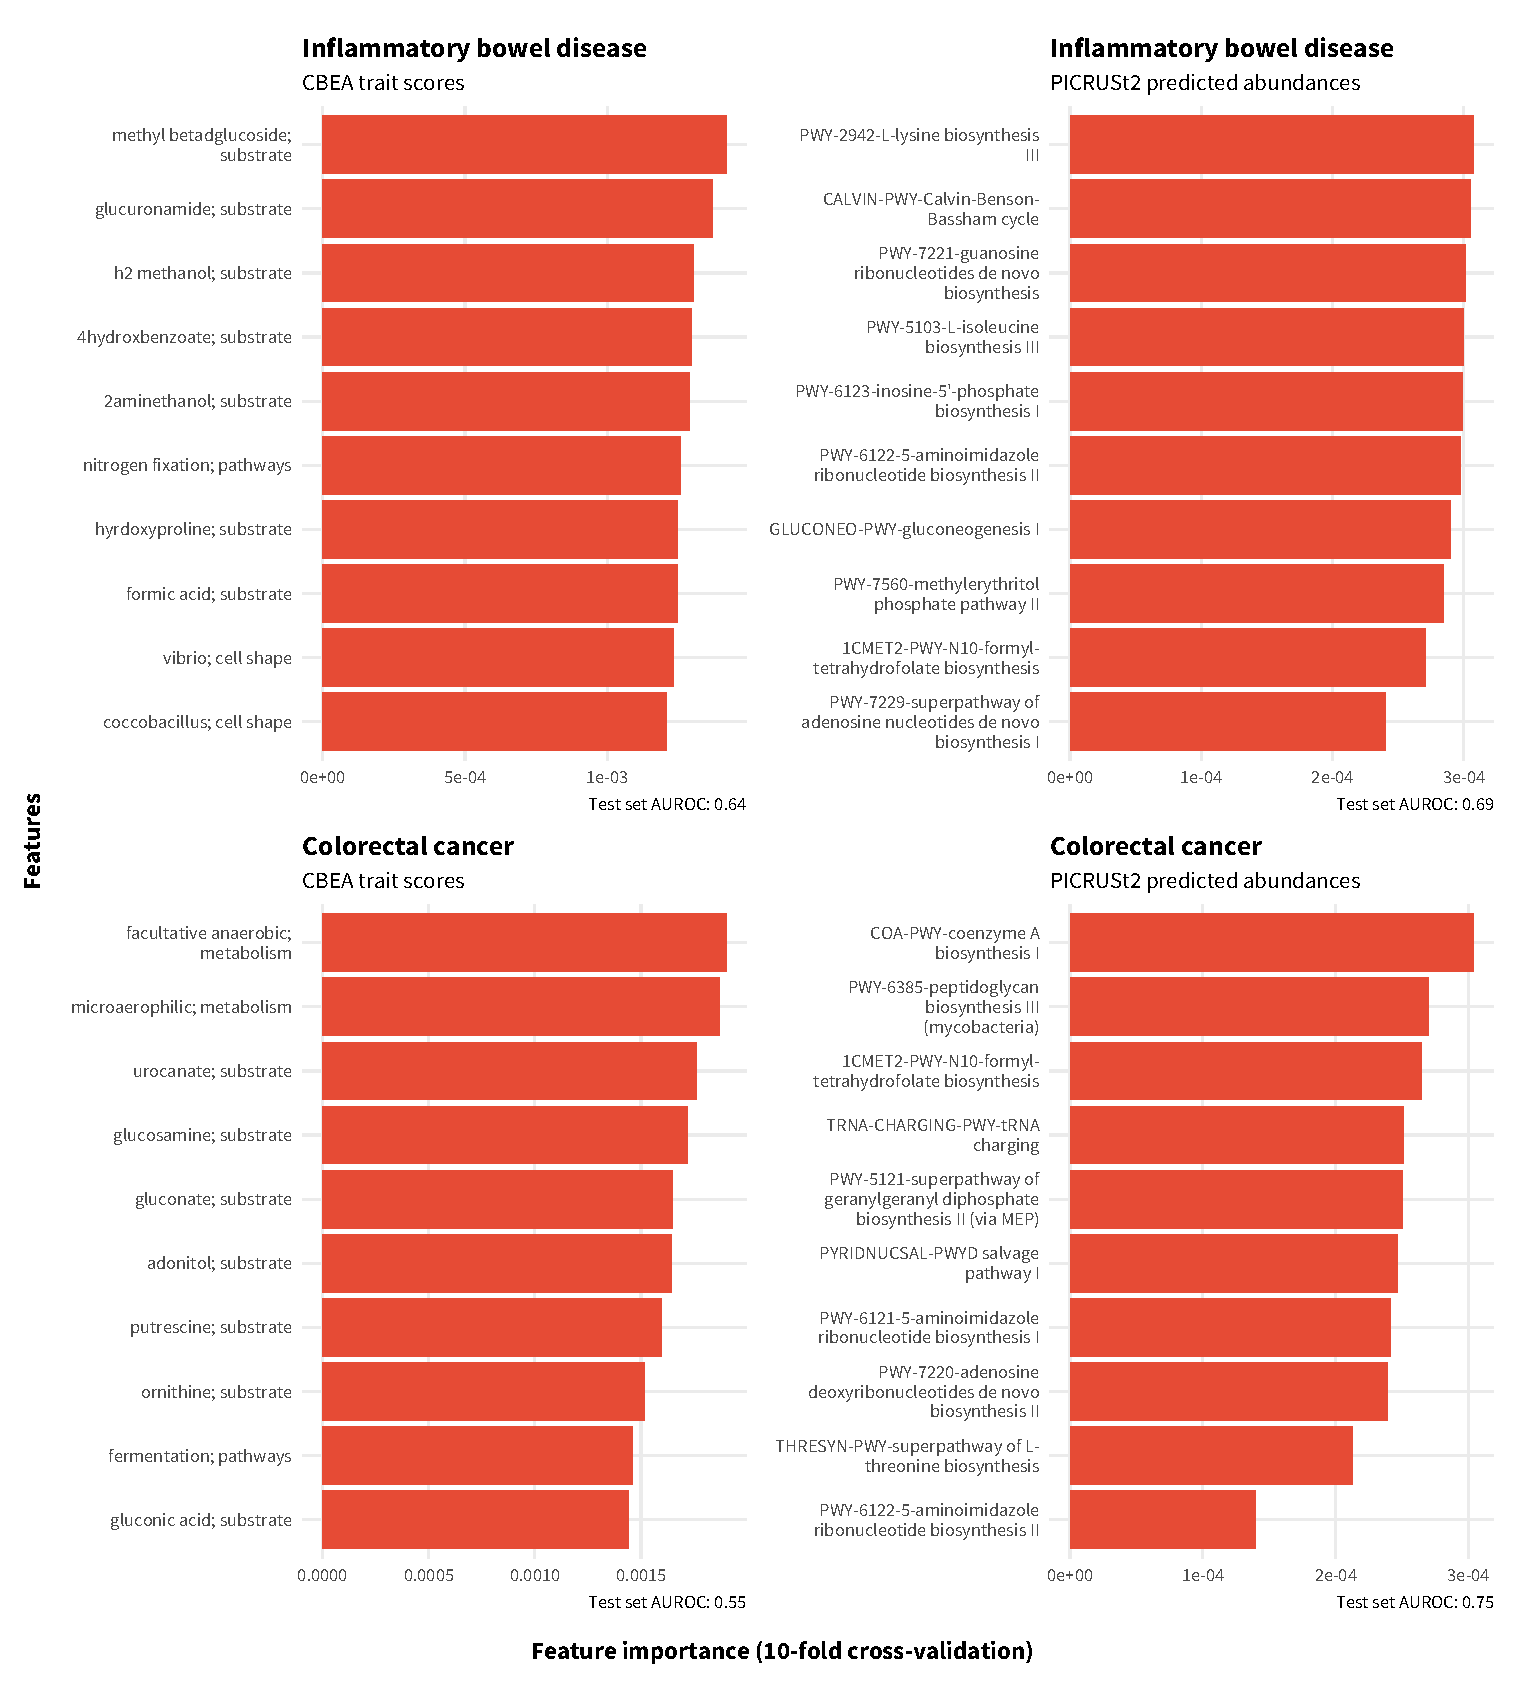
\includegraphics[width=\linewidth]{figures/appD_fs2.eps}
    \caption[Top 10 important features based on random forest model fitted different inputs from data sets profiled with 16S rRNA gene sequencing]{Top 10 important features based on random forest model fitted different inputs from data sets profiled with 16S rRNA gene sequencing. Features were selected from mean decrease in Gini impurity averaged across 500 decision trees and 10-fold cross-validation (nested with the training set) as implemented in \texttt{scikit-learn}. AUROC scored on a held-out test set is also presented for each input type and disease condition.}
    \label{fig:d2}
\end{figure}